%%%%%%%%%%%%%%%%%%%%%%%%%%%%%%%%%%%%%%START PREAMBLE THAT IS THE SAME FOR ALL EXAMPLES
\documentclass{article}

%Required: You must have these
\usepackage{Sweave}
\usepackage{graphicx}
\usepackage{tabularx}
\usepackage{hyperref}
\usepackage{natbib}
\usepackage{pdflscape}
\usepackage{array}
\usepackage{authblk}
\usepackage{gensymb}


%\usepackage[backend=bibtex]{biblatex}
%Strongly recommended
 %put your figures in one place
%\SweaveOpts{prefix.string=figures/, eps=FALSE} 
%you'll want these for pretty captioning
\usepackage[small]{caption}

\setkeys{Gin}{width=0.8\textwidth} %make the figs 50 perc textwidth
\setlength{\captionmargin}{30pt}
\setlength{\abovecaptionskip}{10pt}
\setlength{\belowcaptionskip}{10pt}
% manual for caption http://www.dd.chalmers.se/latex/Docs/PDF/caption.pdf

%Here's how to do that
\topmargin -1.5cm  
\oddsidemargin -0.04cm 
\evensidemargin -0.04cm % same as oddsidemargin but for left-hand pages
\textwidth 16.59cm
\textheight 21.94cm 
%\pagestyle{empty}  % Uncomment if don't want page numbers
\parskip 7.2pt   % sets spacing between paragraphs
%\renewcommand{\baselinestretch}{1.5} 	% Uncomment for 1.5 spacing between lines
\parindent 0pt% sets leading space for paragraphs
\usepackage{setspace}
%\doublespacing
\renewcommand{\baselinestretch}{1.8}
\usepackage{lineno}
 
%%%%%%%%%%%%%%%%%%%%%%%%%%%%%%%%%%%%%%END PREAMBLE 

%Start of the document
\begin{document}

%\SweaveOpts{concordance=FALSE}
\Sconcordance{concordance:sm_doc.tex:sm_doc.Rnw:%
1 223 1}


\bibliographystyle{../../Bibliography/bibstyles/amnat.bst}
\title{Drier soils delay plant phenology across climate change experiments in temperate forest and grassland systems} 
\author[1,2,a]{A.K. Ettinger}
\author[3,b]{J.S. Dukes}
\author[4,c]{M.R. Johnston}
\author[5,d]{C.R. Rollinson}
\author[1,4,6,e]{E.M. Wolkovich}

\affil[1]{Arnold Arboretum of Harvard University, Boston, Massachusetts 02131, USA}

\affil[2]{The Nature Conservancy,Seattle, Washington, USA}


\affil[3]{Carnegie Institute}

\affil[4]{University of Iowa}

\affil[5]{The Morton Arboretum, Lisle, Illinois 60532, USA}

\affil[6]{Forest \& Conservation Sciences, Faculty of Forestry, University of British Columbia, Vancouver, BC, Canada}

\affil[a]{Corresponding author; email: ailene.ettinger@tnc.org; phone: 781-296-4821; mailing address: 74 Wall Street. Seattle, WA 98121, USA }

\date{\today}
\maketitle 
\textbf{Author contributions}: All authors conceived of this manuscript, which began at a Radcliffe Exploratory Seminar in 2016, and all authors contributed to manuscript revisions. AKE and EMW conceived of the idea for the literature review, database compilation, and related Radcliffe Exploratory Seminar, and wrote the manuscript. AKE compiled the datasets; AKE analyzed the data and created the figures.

\textbf{Data Accessibility} 
The data reported in this paper are from the MC3E and the new ExPhen databases, which are both available at KNB \citep{ettinger2018,ettinger2022}. 

\textbf{Running title} Drier soils delay phenology

\textbf{Key words (6-10)} global warming, warming experiment, microclimate, phenology, bud-burst, leaf-out, flowering, fruiting, senescence 


\textbf{Paper type} `Research Article' for \textit{Global Change Biology} %then New Phytologist or Am Bot

\textbf{Number of words in abstract (300 or less)}: 221 

\textbf{Number of words in main text (8000 or less inIntroduction, Materials and Methods, Results, Discussion, and Acknowledgements)}: 


\textbf{Submission Questions} In lieu of a cover letter, authors must answer the following questions during submission (max 250 characters with spaces per answer):
\begin{enumerate}
\item What scientific question is addressed in this manuscript?
\item What is/are the key finding(s) that answer this question?
\item What are the novel results, ideas, or methods presented in your work?
\item Describe how your paper fits within the scope of GCB; What biological AND global change aspects does it address?
\item What are the three most recently published papers that are relevant to this manuscript (include DOIs)?
\end{enumerate}

%%%%%%%%%%%%%%%%%%%%%%%%%%%%%%%%%%%%%%%%%%%%%%%%%%%

%%%%%%%%%%%%%%%%%%%%%%%%%%%%%%%%%%%%%%%%%%%%%%%%%%%

\linenumbers

\section*{Abstract} 
Previous meta-analyses of phenology responses to climate change have focused largely on temperature as a driver of observed shifts. Yet climate change also affects soil moisture, which is limiting to many biological responses. Here we synthesize microclimate and phenology data from climate change experiments in temperate systems---both forests and grasslands---to quantify how soil moisture interacts with temperature to affect plant phenology. 
We find that phenology (budburst, leafout and flowering) delays in drier soils, with the largest delays seen in budburst (-52.2 days per percent reduction in soil VWC). Effects of soil moisture were much smaller than for temperature (-1.7 versus -7.9 in standardized units), with interactive effects of temperature x moisture even smaller (0.5). However, there was high variability in the response across species. Forecasting shifts in soil moisture with warming, we find that soil moisture declines of 10\% would have important effects on the phenology of some species, potentially muting advances due to warming alone. Our results show that soil moisture plays an important role in the phenology of temperate systems, with varying effects across species, and thus is likely to alter ecosystem functions tied to phenology at fine spatial scales. Incorporating local context, including relevant species and downscaled climate change projections, will be critical for planning appropriate management and conservation.

\newpage
\section* {INTRODUCTION} 
\par Climate change is affecting organisms by altering conditions such as temperature and soil moisture around the world \citep{parmesan2006,chen2011}. Some of the most widespread biological responses to climate change are shifts in phenology, the timing of recurring biological events, which have occurred at rates of 2.3-5.1 days per decade \citep{parmesan2006,poloczanska2013,root2003}. Shifts in plant phenology are the most widely documented, with spring phenology (budburst, leafout, and flowering) occurring earlier in recent years \citep{wolkovich2012}, and senescence occurring later \citep{taylor2008,delpierre2009}. 
\par Phenological shifts are typically attributed to warming temperature, a known and well-studied driver of plant phenology. The timing of spring budburst, for example, depends on temperature through both chilling (the prolonged exposure to cold temperatures after growth cessation in the fall) and forcing (exposure to warm temperatures). Forcing effects are typically considered more dominant, so much so that many models use only forcing to predict phenology. These include common models of `growing degree days' (GDD) in which phenological events are triggered after a certain thermal sum is reached \citep[e.g., ][]{olsson2014process}. Recent trends of advancing spring phenology may be due to increases in chilling and/or forcing with global warming \citep{fujisawa2010, ibanez2010,cook2012b}. %In places where delays in spring phenology have occurred, reductions in winter chilling are often the attributed cause \citep{yu2010}.

\par Effects of changing patterns of precipitation and soil moisture on plant phenology have received less attention, but documented in some cases. Many climate change experiments have focused on the effects of altered precipitation regimes, with meta-analyses highlighting the diversity of findings \citep{lu2023contrasting}, and the importance of interactive effects of precipitation shifts with global change drivers \citep{zhou2023climate}. In particular, recent work suggests warming combined with drought treatments may slow advances in phenology \citep{zhou2023climate}. Budburst can be slowed by water stress through inhibiting cell elongation \citep{essiamah1986}, and growing season start may be delayed by drought in grasslands \cite{cui2017}. Conversely, flowering phenology can be advanced by drought conditions \citep{hamann2018}. Effects of soil moisture on phenology have been most well- quantified in arid and grassland ecosystems \citep[e.g., ][]{essiamah1986,reich1984, van1993, tao2019}; the role of soil moisture on phenology in other ecosystem types, especially more mesic ones, is less explored. 

\par Recent studies have suggested that moisture may play an important---but complicated---role in the phenology of temperate ecosystems as climate change progresses \citep[e.g.,][]{seyed2018,wang2022}. For example, \citet{wang2022} found that decreasing precipitation frequency correlates with earlier leafout in many regions, while others have found variation in moisture sensitivity across ecoregions \citep{seyed2018}. Increasing research using large-scale observational phenology data (e.g., remote sensing products such as NDVI) has documented an important role for soil moisture from forests to grasslands \citep{lian2020summer,shen2022plant,liu2024soil}, and suggested temperature may play a role through moderating soil moisture \citep{liu2024soil}. Teasing out the role of soil moisture from temperature is challenging through long-term climate trends alone, however. Perhaps unsurprisingly then, many studies have attempted to manipulate moisture via experimental precipitation or drought treatments \citep[e.g.,][]{morin2010,hoeppner2012,rollinson2012b,clark2014a}, though few experiments have directly reported on moisture effects of phenology in temperate, non-arid and non-crop systems. Effects in more arid systems are diverse, often with no overall shift in phenology \citep[e.g.,][]{sherry2007,de2017challenging,howell2020}, suggesting that identifying clear trends from single experiments may be difficult. 

\par Field-based climate change experiments that warm plots to different levels and apply precipitation or drought treatments are valuable tools to study effects of temperature and moisture on plant phenology, and can be leveraged for additional insights through synthesis across studies. Experiments can combine temperature and precipitation treatments to decouple them compared to what may be observed in nature, allowing their effects to be more robustly quantified. Further, these treatments allow for studying effects of ``no-analog" climate scenarios forecasted for the future, particularly when they employ active-warming methods, such as forced air heaters, soil warming cables, or infrared heaters \citep{shaver2000,williams2007b,aronson2009}. Climate change experiments can monitor daily soil moisture and air temperature at the plot-level, allowing detailed quantification of how microclimate affects plant phenology \citep{ettinger2019}. While previous meta-analyses of phenology in climate change experiments have focused primarily on effects of temperature \citep[e.g.,][]{wolkovich2012a}, there has been little synthetic work on moisture effects across experiments. 
\par Here we use measured microclimate and phenology data across experiments to test how soil moisture and above-ground temperature together affect plant phenology (budburst, leafout, flowering). Our aims were to: (1) quantify effects of soil moisture versus temperature alone and synergistically across species; (2) evaluate how consistent effects were across species, functional groups and biomes (forest versus grassland), and (3) forecast effects to understand future implications of moisture shifts with warming for phenology. 

\section* {MATERIALS AND METHODS}
\textbf {\emph{Data}}-- To investigate how soil moisture interacts with temperature to affect phenology, we used two databases that compiled data from climate change experiments. Microclimate data came from the MicroClimate from Climate Change Experiments (MC3E) database \citep{ettinger2018, ettinger2019}. Phenology data came from a ExPhen, a new database of phenology from climate change experiments \citep{ettinger2022}. 
\par Both databases were created by first identifying published, active-warming field experiments, many of which included precipitation manipulations. We focused on \textit{in situ} active-warming manipulations because recent analyses indicate that active-warming methods are the most controlled and consistent methods available for experimental warming \citep{kimball2005,kimball2008,aronson2009,wolkovich2012a}. We carried out a full literature review to identify potential active-warming field experiments, following the methods and search terms of \citet{wolkovich2012a} for their Synthesis of Timings Observed in iNcrease Experiments (STONE) database \citep{wolkovich2012}, but restricting our focus to active-warming experiments. Further, because our goal was to tease out variation in microclimate (including temperature and soil moisture), we focused on warming studies that included multiple levels of warming and/or precipitation treatments. These additional restrictions constrained the list to 11 new studies published after the STONE database, as well as six of the 37 studies in the STONE database. We contacted authors to obtain daily microclimate and phenological data for these 17 studies and received data (or obtained publicly available data) for 10 of them, as well as datasets from five additional sites offered or suggested to us over the course of our literature review and data analysis. The daily temperature and soil moisture data from these 15 experiments comprise the MC3E database \citep{ettinger2018,ettinger2019}. Of these, we were able to obtain plot-level phenology data from 14 experiments, which comprise the ExPhen database of experimental phenology, available at KNB \citep{ettinger2022}. 
\par Here, we analyze phenology data from the eight experiments in ExPhen that contain both regularly monitored plot-level soil moisture and above-ground temperature data (Table S1). Because we wished to examine variation among species and across sites, we focus on the most common phenophases monitored, which were measured in three or more different experiments: budburst, leafout, and flowering. Two of the eight experiments were located in grassland ecosystems; the remaining six were in forests (Table S1). The database is species-rich, including 41 species monitored for budburst across five sites, 137 for leafout (across five sites), and 124 for flowering (across all eight sites), for a total of 190 species. These species span grasses (16 species), forbs (109 species), shrubs (29 species), and trees (36 species). 

\par\textbf {\emph{Analysis}}--
To understand how soil moisture interacts with temperature to affect phenology, we fit models with microclimate predictor variables of measured soil moisture, measured above-ground temperature, and their interaction to phenology response data (budburst, leafout, flowering day of year). We excluded conifers from the analysis, because their phenology has distinct differences from angiosperm phenology \cite{polgar2014} and conifer data existed from only one site in the database. For all phenophases, the response variable was day-of-year of the phenological event. 
\par Predictors for our primary models were measured plot-level above-ground temperature, soil moisture, and their interaction. We chose to use measured microclimate as explanatory variables, rather than categorical treatment levels or target warming level, in our meta-analysis because experimental treatment effects from warming and drought can interact to alter microclimate conditions, in part due to feedbacks between temperature and soil moisture conditions \citep{ettinger2019,mcdaniel2014}.
 
\par We used hierarchical Bayesian models to test for effects for each species, as well as an overall effect, while accounting for site, year and plot-level effects. Grouping factors (often called `random effects') for all phenology models were species (with random slopes and intercepts), site (random intercept), and year nested within site (random intercept). We fit models using the programming language \texttt{Stan} \citep{Carpenter:2016aa} (\texttt{www.mc-stan.org}), accessed via the \texttt{brms} \citep{burkner2021} package in R \citep{rcoreteam2022}, version 4.1.3. For each model fit, we ran four chains simultaneously, each with 4 000 iterations (2 000 of which were used for warm-up). Equations for these models can be found in the Supplemental Methods. 

\par Given our aim to directly compare moisture and temperature effects, we used standardized predictors, which have an added benefit of improving model stability \citep{gelman2007}. Standardizing predictors is a common technique in regression analysis; here we z-scored predictor variables (subtracting the mean and dividing by the standard deviation) and report coefficients from standardized predictor models as per SD (standard deviation), alongside estimates of coefficients in their natural units. 
\section* {RESULTS}
\par We found that both higher soil moisture and higher temperatures advance phenology, meaning two common effects of warming experiments---soil drying and warming---have contrasting effects on phenology. We found that soil drying delays phenology and warming temperatures advance phenology. For budburst, wetter soils and warmer temperatures alone advanced phenology by -1.7 per SD of soil moisture  (or -5.22 days per 10 percent increase in volumetric water content) and -7.9 per SD of temperature (-3.4 per degree Celsius), respectively. We did not find evidence of strong interactive effects of soil moisture and temperature on phenology: together, wetter and warmer conditions delayed budburst only a small amount (interaction effect of 0.5 per SD [95\% uncertainty intervals: -0.6 to 1.4] or 3.7 natural units). 
\par The magnitude of soil moisture effects varied across phenophases, with effects on budburst being stronger than those on leafout (-0.4 per SD of soil moisture) and flowering (-1.3 per SD). Similar to budburst, temperature effects were stronger than soil moisture for leafout (for which the temperature effect was -10.3 per SD) and flowering (for which it was -7.9 per SD), across all species (Fig \ref{fig:bblofl}). Estimates of interactions between soil moisture and temperature on phenology also varied by phenophase, with weak positive interactive effects estimated for leafout (0.5) and budburst (0.5) and a stronger but negative the interaction for flowering (-1.1). This negative interaction implies that there may be synergistic effects of soil moisture and temperature (both of which also have negative estimated effects on flowering), resulting in flowering that advances even more strongly than would be expected by simply adding together the  estimated effects of temperature and  moisture each acting alone. 

\par These overall effects varied widely across species (Fig \ref{fig:bblofl}). Species-level variance for the effect of moisture was 2.7 standardized units for budburst, 3.8 for leafout, and 3.8 for flowering. Species-level variance was even greater for temperature effects: 11.4 for budburst, 10.3 for leafout, and 6.2 for flowering. Species-level variability in responses to moisture was not predictable by life form (trees, shrubs, herbs, grasses, Fig. \ref{fig:forms}, column 2)  nor by ecosystem (grassland versus forests, Fig S2), across the three phenophases we studied. We did observe more negative effects of temperature on trees compared to shrubs for budburst, and on both trees and grasses compared to shrubs and forbs for leafout (Fig. 2, column 1). Interactions between temperature and moisture effects on leafout also seemed to skew more positive for grasses compared to other life-forms (Fig. 2, column 3)
\par We applied the above budburst model to forecast possible effects of climate change on phenology. Based on the estimated effects, wetter soils advanced spring budburst at a rate of 5 days per 10\% increase in soil volumetric water content (VWC). Thus, if soil moisture is reduced by 10\% of its current state, as is expected over the next 50 years in areas where many of the experiments were conducted (the northeastern United States) \citep{berg2017} (moving from, e.g., 21.5\% VWC -- the mean value for January-March across all sites for which budburst was monitored -- to 19.4\% VWC), budburst would be delayed by approximately 1 day on average, due to changes in soil moisture alone (Fig \ref{fig:bbsp}).
%\item \textbf{Soil moisture effect size is bigger in full dataset than in controls only, for BB.} Mean and range of SM is similar (though max is a bit higher in full dataset; min is similar).
%\item \textbf{Effects of climate manipulations on temperature and soil moisture}

%\par Mean annual soil moisture is negatively affected by target temperature treatment, and positively affected by precipitation treatment. (Figure \ref {fig:soilmois}). These effects varied by site; for example, at exp07 soil moisture was positively affected by temperature treatment. Air temperature is positively affected by target temperature treatment, and negatively affected by precipitation treatment. (Figure S\ref {fig:temp}).

\section* {DISCUSSION}
\par We have synthesized climate change experiments to find that soil moisture affects plant phenology in temperate non-arid ecosystems, in addition to the arid ecosystems where effects of water availability on phenology have been more often reported \cite[e.g.,][]{reich1984,van1993,cleverly2016soil,bertiller1991seasonal}. This offers new insights because there has been little synthetic research across experimental sites to understand impacts of soil moisture on phenology, despite the reality that many experiments collect these data. Soil moisture has not been a focus of previous phenology meta-analyses \cite[e.g.,][]{wolkovich2012}, nor of most multi-species phenology studies in temperate mesic grasslands and forest ecosystems \cite[e.g.,][]{Vitass2021}, Our work helps develop robust, experimental evidence that builds on large-scale observational research that increasingly suggests an important role for soil moisture in phenology \cite[e.g.,][]{}. It also builds on small-scale experiments, which have found impacts of precipitation on phenology \cite[e.g.,][]{currier2022precipitation}. Our findings highlight that, in mesic grasslands and forests, too, plants need water to advance budburst, leafout, and flowering; the delaying effect of dry soils suggest that moisture can be a hidden, but potentially limiting, factor affecting phenology in temperate systems not typically thought to be water-stressed. 

\par Soil moisture is and will continue to shift with climate change \citep{berg2017}, so while we found soil moisture had a smaller effect size than temperature, it could have a big impact on phenology. Some areas, such as the northeastern United States (where many of the experiments were conducted) are getting wetter, and other places are expected to get drier \citep{berg2017}. Overall, our forecasting suggests that temperature will continue to be a dominant controller of phenology, but that soil moisture also matters, especially for certain species. 
%\par \textbf {High variation in responses to soil moisture across species and phenophases}
\par Despite the overall delaying effect of soil drying we quantify for phenology, our results suggest that forecasts will need to contend with high variation in species responses, as well as differences across phenophases \ref{fig:}. There do not appear to be strong differences in soil moisture effects across broad functional types, though we observed some differences across functional groups in temperature leafout responses, in which grass and tree responses appear more negative than those of forbs and shrubs, Fig. \ref{fig:forms}). More positive interactive effects of soil moisture and temperature are also apparent for grasses compared to other groups.  
\par Our results that broad functional types do not systematically respond differently to soil moisture, temperature and their interaction contrasts with some findings \citep[e.g.,][]{rollinson2012,castillioni2022effects}, but supports growing work suggesting that species traits may be far more predictive \cite[e.g., ][]{diaz2016global}. Major traits related to root and leaf structure can impact species' drought tolerance. For trees, traits related to drought tolerance may co-vary with frost-risk, as ring-porous species are generally more drought-tolerance but risk greater damage from spring frosts compared to diffuse porous species \citep{bader2022less,wang2022contrast}; not surprisingly ring-porous species leafout later then diffuse-porous species \cite{lechowicz1984}. Such interconnections between phenology and other traits occur in other systems, too \citep[e.g.,][]{ocheltree2020identification}, and suggest the potential for a framework to better predict the high variability of responses across species \citep[e.g.,][]{morales2024phylogenetic}.

\par Our findings that sensitivity to soil moisture and interactions with temperature vary across phenophases align with other recent studies. \citep{buonaiuto2021differences}, for example, also found varying sensitivity of flower and leaf phenology to environmental cues, even within species. In our study, variability across species in the soil moisture response was lowest for budburst (2.7 compared to 3.8 for leafout and  3.8 for flowering), perhaps suggesting that, across species, soil moisture is a key control on timing of budburst (e.g., by affecting cell elongation \citep{essiamah1986}). The direction of interactive effects of soil moisture and temperature also varied in sign across phenophases, with weak positive estimates for budburst and leafout, and stronger positive interactive effects for flowering (Fig. \ref{fig:bblofl}). Thus, the implications of climate change driven shifts in soil moisture for phenology are likely to depend on when during the growing season shifts are greatest and, especially for flowering, how it intersections with temperature shifts, among other factors. Such shifts are likely to affect fitness, as well, with some species more strongly affected than othersm thus scaling up to impact community structure and function, as \citep{buonaiuto2021differences} also suggest.
%\par Our findings of variation in soil moisture effects across species and phenophase may explain inconsistencies observed in previous studies. For example, \cite{wolkovich2012} found that exotic species advance with precipitation, whereas native species delay at one site (Fargo). 

%\textbf {Forecasting multiple drivers}
\par The experimental data we synthesize here highlight that multiple drivers that are shifting with global change affect phenology and are important for accurate forecasts. Highly-cited phenology research in temperate grassland and forest systems has frequently ignored effects of soil moisture and other drivers, focusing instead on temperature. Our finding that soil drying has an overall delaying effect on phenology is consistent with \citet{seyed2018}, who found that moisture deficit generally delays phenology in forest ecosystems, and with recent experimental \citep{liu2022} and observational \citep{tao2020} studies in temperate grasslands. Our results align within a larger literature from other systems that have found moisture matters to phenology, including alpine systems dominated by snowpack \citep[e.g.,][]{dunne2004,sherwood2017}, and arid/semi-arid ecosystems where precipitation is known to be more limiting \citep{tao2019}. 
\par Forecasting phenological shifts with global change also, then, depends on integrating multiple drivers. Soil moisture, temperature, and their interactions were our focus here but other global change factors intersect to affect phenology. CO2, for example, and soil moisture may actually mediate plant phenology responses to warming and nitrogen addition \citep{liu2022}.

%\textbf {Implications and next steps}
\par To do this forecasting, we need to improve how we relate experiments to the `real world'. This includes moving beyond treatments levels to analyze plot-level microclimate- closer to how plants may be experiencing treatments. Our study differs from some because we used field-measured soil moisture -- most studies use precipitation \citep[e.g.,][]{tao2020} or gridded moisture products \citep[e.g.,][]{tao2019}. The problems with these proxies are widely known, including challenges with validation at fine spatiotemporal resolutions, though a number of new products are available and seem promising \citep{peng2021roadmap,brocca2024exploring}. However, our use of measured soil moisture also created a data limitation, as we were able to use only a subset of all the climate change experiments included in the ExPhen and MC3E databases. Increased measurement, reporting, and sharing of environmental conditions-- including soil moisture and temperature-- could help to disentangle how temperature is affected by soil moisture, and how soil moisture is affected by temperature treatments.
\par The soil moisture-phenology relationships we quantify within species may scale up and interact with other factors to affect ecosystem-level functions such as biomass and carbon uptake or storage. Disentangling effects from climate versus soil can be challenging but has demonstrated the importance of species interactions and multiple limiting nutrients in vegetation responses to global change \citep{wilfahrt2021}. In addition to playing a role in  budburst, leafout, and flowering phenology, for example, soil moisture affects plant resorption of nitrogen and phosphorus during leaf senescence\citep{estiarte2022}. Shifts in soil moisture and cascading effects on phenology may ultimately lead to changes in growing season length and carbon uptake (cite grephon?), especially since soil moisture is a key control of nutrient cycling, including nitrogen and carbon \citep{liu2019soil}.

\section* {Conclusions}
Now underway for four decades, climate change experiments \citep[e.g.,][]{tamaki1981,carlson1982,melillo2017} can provide a unique opportunity to disentangle multiple drivers and understand biological responses to climate change. Yet the full range of changes in environmental conditions imposed by these experiments is rarely presented. Using two databases that compile microclimate data and phenologyical responses from multiple warming experiments we show that soil moisture, in addition to temperature, affects plant phenology. We quantified phenological delays with soil drying across budburst, leafout, and flowering that suggest these effects should be more often included in modelling and forecasts of seasonal shifts with climate change. Given that the magnitude and direction of the response varied across species, and that projected shifts in soil moisture with climate change vary spatially, specific implications of our findings-- e.g., whether incorporating shifts in moisture results in more muted or exagerated phenological shifts than would be expected based on temperature along- will depend on local context. Incorporating these findings with locally relevant biological and climate information can be used to assess biological impacts of climate change and manage natural resources for enhanced climate resilience.
%\citep{tao2019} "However, effects of precipitation and soil moisture on BBD varied among [herbaceous] species [in Inner Mongolia grassland]." ... "correlations between BBD and SM were negative, suggesting that greater soil moisture would result in an earlier BBD." and it seems like mostly they did not find correlations otherwise; also their data are a gridded product
%\citep{howell2020} "Altered precipitation treatments were only applied in early years of the study and neither precipitation treatments nor the treatments’ legacies significantly affected B. tectorum phenology." But warming did advance flowering and shorten the vegetative season. % https://www.frontiersin.org/articles/10.3389/fpls.2020.570001/full

%\par Altough soil moisture is expected to shift with climate change \citep{berg2017}, it has not been a focus of previous meta-analyses \cite[e.g.,][]{wolkovich2012}. Thus, our finding that soil moisture affects phenology, across the experiments in commmonly studied temperate forest and grassland ecosystems (i.e., those included the ExPhen database, Table \ref{tab:studylocs}, Fig. \ref{fig:map}), may surprise some. Soil moisture has been investigated frequently in arid or semi-arid ecosystems (e.g. CITE), including experiments that find either no effects (cites) or contrasting results across species (cites). Effects of moisture or precipitation on phenology have been extensively studied in alpine systems dominated by snowpack, as well, where less snow generally advances phenology \citep[e.g.,][]{dunne2004,sherwood2017}. 


% could also connect to observational studies finding differences among ecoregions where species also differ (see end of doc, where I added some notes). Could stress our results mean we need to understand the drivers of these species-level differences better...

\section* {Acknowledgements}

We are grateful to those who shared their experimental climate data with us, allowing it to be included in the MC3E and ExPhenvdatabases. We thank the Radcliffe Institute for Advanced Study at Harvard University, which provided funding for an Exploratory Seminar at which the ideas in this paper were conceived. This research was also supported by the National Science Foundation (NSF DBI 14-01854 to A.K.E.). Any opinion, findings, and conclusions or recommendations expressed in this material are those of the authors and do not necessarily reflect the views of the National Science Foundation.

\bibliography{mylibrary.bib}

\section*{Figures}


\begin{figure}[h]
\centering
 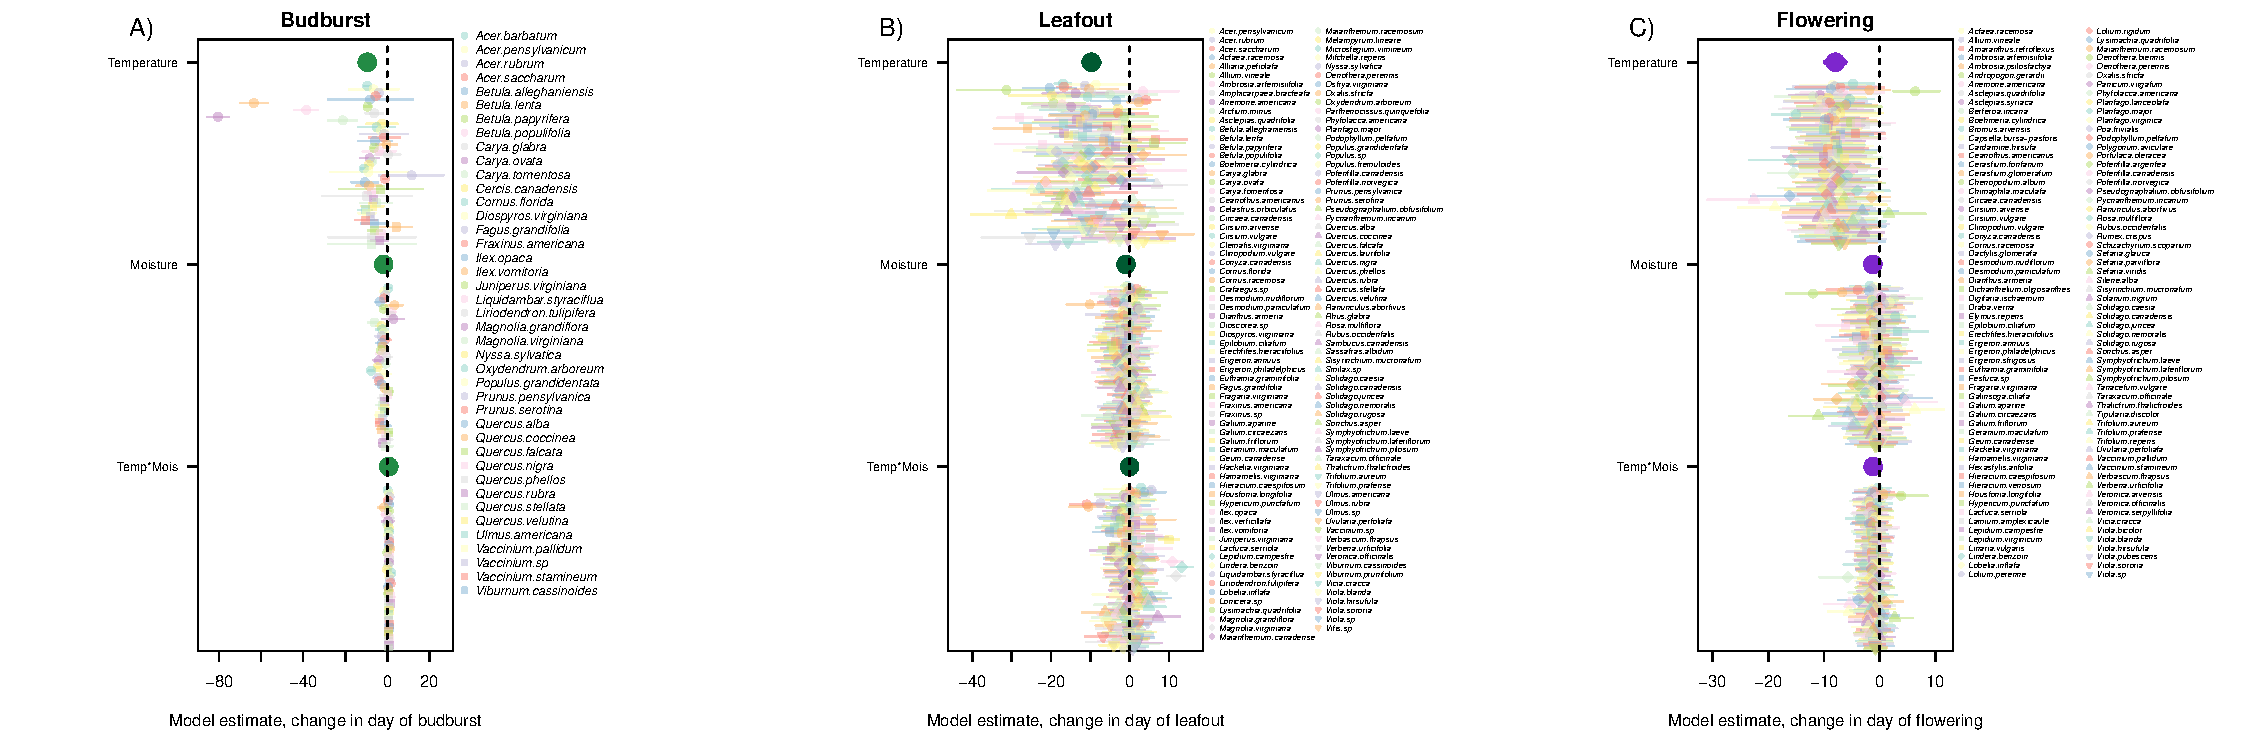
\includegraphics{../../Analyses/soilmoisture/figures/m5_bbdlofl.pdf}
 \caption{\textbf{Model coefficients from budburst, leafout, and flowering models (with centered predictors)} and including all species. We could show only the most common species here, to improve readability, and then show this version (with full species list) in the supplement. Thoughts?} 
 \label{fig:bblofl}
 \end{figure}
 
\begin{figure}[h]
\centering
 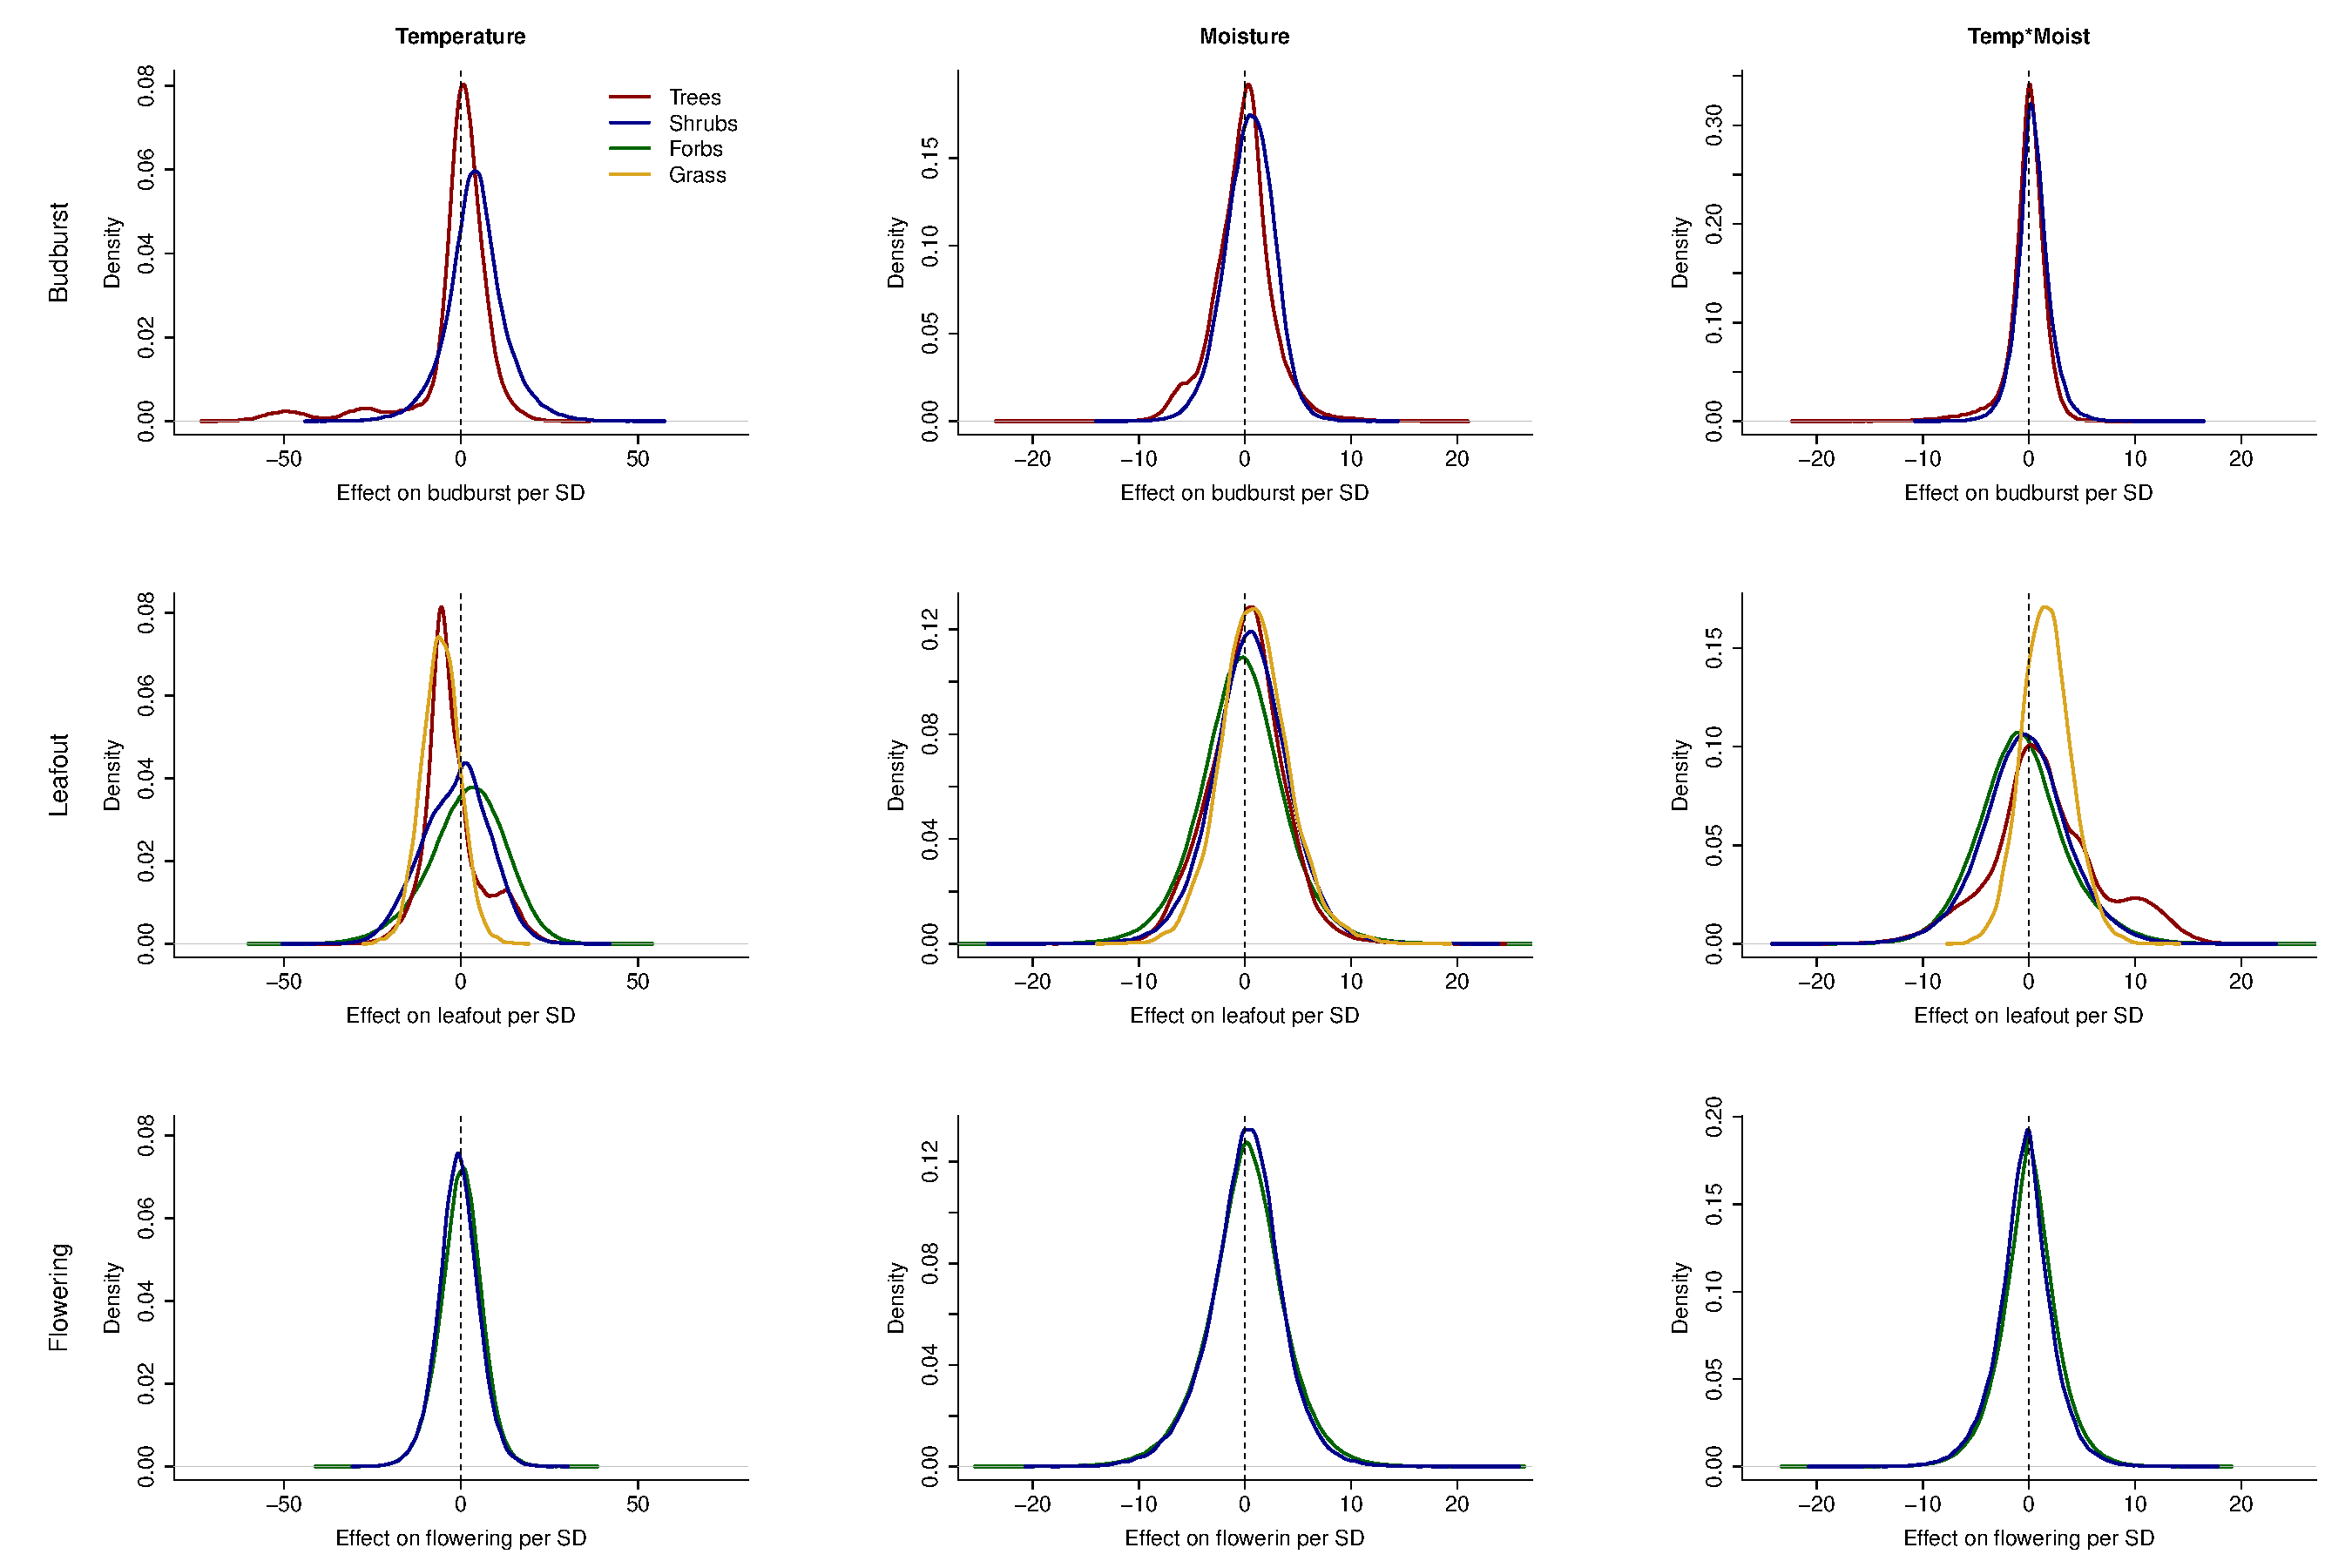
\includegraphics{../../Analyses/soilmoisture/figures/curvebbloflform_widexaxis.pdf}
  \caption{\textbf{Effects of temperature, soil moisture, and their interaction summarized life forms} reveal minimal differences in estimated responses to soil moisture (middle column). Curves show probability density functions for posterior samples of estimated effects for temperature, soil, and their interaction summarized by species and grouped into four life forms (trees, shrubs, forbs, and grasses). Patterns do appear to vary by life form for temperature (first column) and interactions (third column).  For budburst, temperature effects were more negative for trees compared to shrubs, and more negative for both trees and grasses compared to shrubs and forbs for leafout. Interactions between temperature and moisture effects on leafout, on the other hand, seemed to skew more positive for grasses compared to other life-forms.}
 \label{fig:forms}
 \end{figure}

 \begin{figure}[h]
\centering
 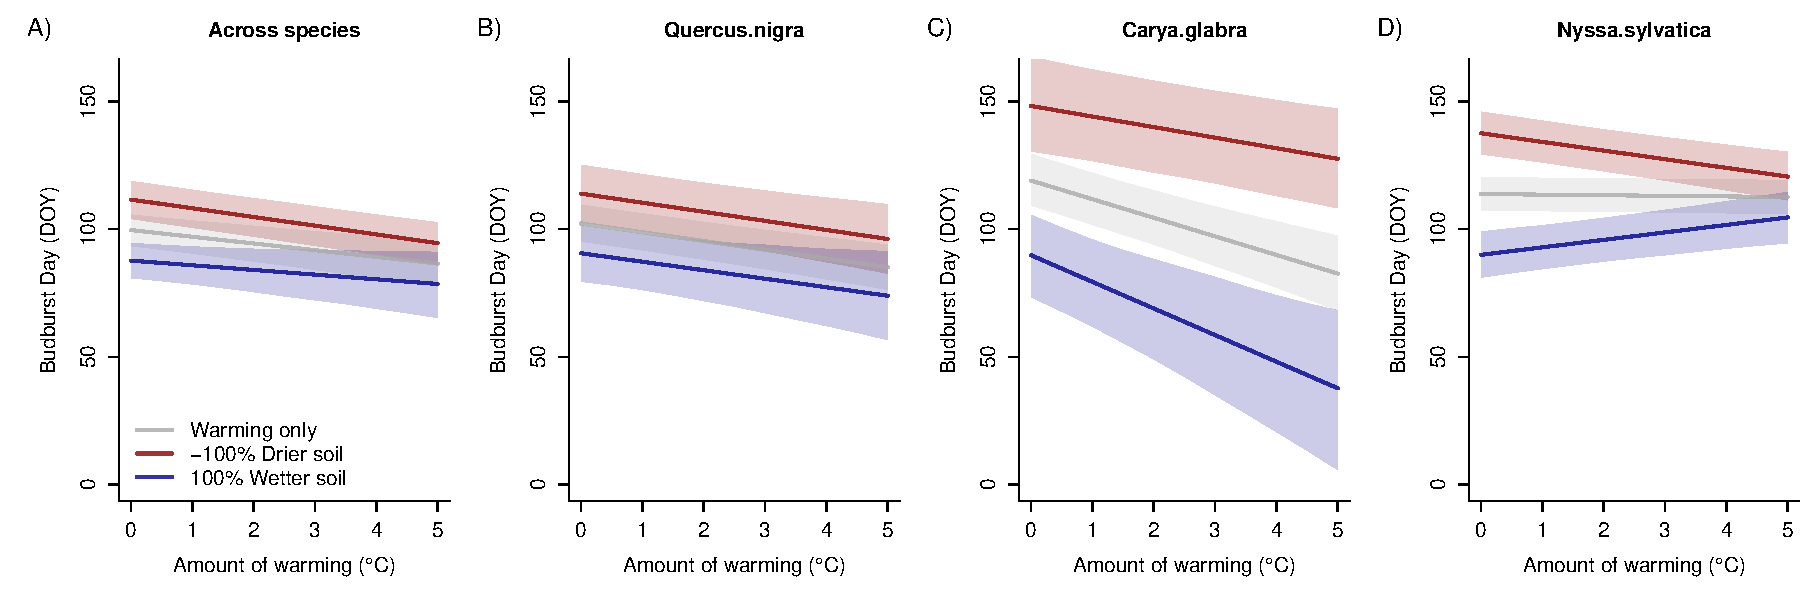
\includegraphics{../../Analyses/soilmoisture/figures/tempforecast_bb_0_5_135_28_105_4_degwarm.pdf}
 
 \caption{\textbf{Patterns of forecasted changes in budburst date with warming and shifts in soil moisture vary across species}. Across all species, our model estimated negative effects (i.e., earlier) of both temperature and soil moisture on budburst and a weak interaction between the two effects (A, and example species \textit{Quercus nigra} in B); however, the magnitude of these effects, as well as the sign and magnitude of the estimated interaction between soil moisture and temperature, differed across species, resulting in divergent patterns with forecasted conditions under climate change. Budburst may occur much earlier in wetter vs drier soils with warming for species that have a synergistic interaction between soil moisture and temperature, such as \textit{Carya glabra} (C). Whereas, other species with an antagonistic interaction, such as \textit{Nyssa sylvatica}(D), may experience delayed budburst in wet soils but advance in dry soils.}
 \label{fig:bbsp}
 \end{figure}

%%%%%%%%%%%%%%%%%%%%%%%%%%%%%%%%%%%%%%%%
\end{document}
%%%%%%%%%%%%%%%%%%%%%%%%%%%%%%%%%%%%%%%%


% Notes on some papers by Lizzie on 22 July 2022 -- on 24 July 2022 I deleted notes I already included above in manuscript. 

\citep{Crimmins:2010lv} "the decrease in autumn precipitation observed over the study period appears to explain the delay in onset observed for many of the species across the elevation gradient."



\cite{cabon2020} Good paper to cite for temperature and moisture being co-limiting .. hmm but they actually say "We found that temperature alone explains the onset of tracheid production" [and this is a modeling paper]


\cite{craine2012} most species flowerisng during warm wet times, but also discusses sort of divergence -- early versus late flowering species

